\section{Search, representation, and output semantics}
\subsection{Norm-primary enumeration}
The implemented search \ev{E3} compiles the three zero residuals
\eqref{eq:as}, \eqref{eq:r3}, and \eqref{eq:r4}, together with the functional
field operations, into a Boolean arithmetic DAG. Field parameters and the
domain basis are fixed inputs. A primary-only decision policy is enforced
in a source-pinned native CryptoMiniSat fork; auxiliary coordinates still
participate in propagation and Gaussian elimination.

\begin{center}
\fbox{\begin{minipage}{0.92\linewidth}
\textbf{Algorithm 1: exact norm-primary enumeration with a budget.}\\
1. Validate the field, curve, target, and domain; require $z\ne0$.
Build the elementary coefficients and the functional parametrization.\\
2. Compile the residuals with the declared affine-support limit.
Initialize the native solver with the primary decision mask.\\
3. On SAT, replay every declared coordinate against its unique functional
extension; check every CNF/XOR relation and the original arithmetic DAG.
Independently form the literal polynomial norm and divide by $X+z$.\\
4. Retain the verified norm witness. Block the entire primary assignment
and repeat. A duplicate or failed replay is an error.\\
5. On native UNSAT, report complete enumeration of this norm-primary
predicate, conditional on solver correctness. On UNKNOWN, a model cap,
or an expired budget, return verified witnesses as a lower bound with the
exact count unset. Keep original-system completeness unset.
\end{minipage}}
\end{center}

Soundness follows from Theorem~\ref{thm:chart} and independent replay.
The full-primary blocking clause removes exactly the emitted assignment.
Induction gives distinct witnesses and no removal of an unreported primary
assignment. Exhaustion of the remaining predicate therefore establishes
coverage within the norm chart, conditional on the solver's UNSAT verdict.
The implementation does not supply an independently checked large UNSAT
certificate; native exhaustion is not advertised as certified generalized
root finding.

There are at most $2^{5d+n+1}$ primary assignments. Exhaustive functional
evaluation is a finite reference method, but this bound is exponential.
The SAT implementation has no established polynomial or subexponential
worst-case advantage. Storage includes the compiled DAG, solver state,
and emitted witnesses; learned-clause growth is not bounded here by a small
polynomial guarantee. Output enumeration itself can require exponential time.

\begin{figure}[tb]
\centering
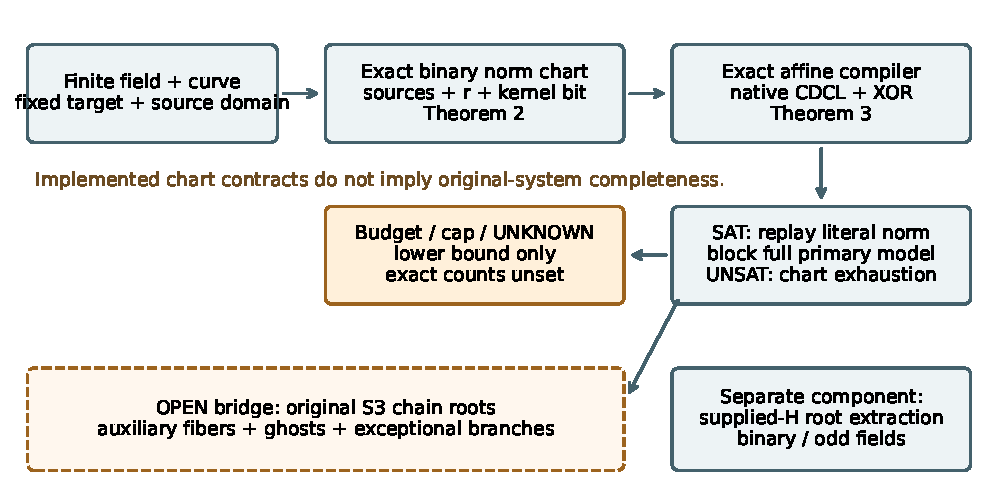
\includegraphics[width=\linewidth]{figures/architecture.pdf}
\caption{Contract boundaries. Exact chart enumeration and supplied-polynomial
root extraction are implemented components. The original-system reconstruction
bridge and an independently certified complete hard search remain open.
An interrupted search returns a lower bound, not an exact count.}
\label{fig:architecture}
\end{figure}

\subsection{Bounded affine cones}
At a binary XOR wire, represent the value as an affine form over already
defined primary atoms, nonlinear outputs, and retained linear atoms.
Addition is symmetric difference of supports, with a separately retained
constant bit. When the declared support limit is exceeded, introduce a
shared parity alias with its exact XOR definition. At an AND retain the
exact three-clause gate definition on signed input aliases and a fresh output.
Constant wires and empty parity contradictions must remain exact.

\begin{theorem}[Unique extension under affine contraction]\label{thm:compiler}
For an acyclic functional Boolean DAG and the transformation just described,
every primary assignment has exactly one extension satisfying the introduced
definitions. That extension has the same final residuals as the original DAG.
Projection of satisfying assignments to primary coordinates is a bijection
between the transformed and original predicates.
\end{theorem}
\begin{proof}
Order the construction topologically. Every new coordinate is defined as a
specified parity or AND of earlier coordinates, so its value exists and is
unique after those coordinates are fixed. Induction proves that every affine
form denotes its original wire value, including the constant phase and
cancellation to an empty support. The same induction applies conversely to
any satisfying assignment of the defining constraints: its new coordinates
must equal those values. Final zero constraints therefore agree exactly,
which proves both directions and uniqueness.
\end{proof}

The support limit controls the representation, not a relaxation of
nonlinear multiplication. Dense affine forms can shrink the number of
external variables while dramatically expanding native internal XOR cuts.
For the pinned two-input cut construction the profile estimates additional
coordinates per row by
$\lfloor\max(\ell-3,0)/2\rfloor$, where $\ell$ is row length \ev{E2}.
This is a source-specific pre-cleaning estimate, not a portable SAT theorem.
Actual post-flush counts are recorded separately. The compiler proof gives
no monotonic relation between either count and solution time.

\subsection{Permutation representatives}
\begin{proposition}[Source symmetry]\label{prop:symmetry}
If all five source domains equal $D$, and the tested predicate depends on
the sources only through $H_x$, sorting the five encoded source coordinates
selects one representative of each source-permutation orbit. Restoring
every distinct permutation, with the remaining primary parameters fixed,
recovers the full ordered norm-primary set.
\end{proposition}
\begin{proof}
The product $H_x$ is invariant under permutations. A fixed total order on
the finite coordinate encoding gives exactly one nondecreasing tuple for
each multiset. Every ordered tuple with this multiset is a distinct
permutation of that representative. These sets are disjoint for different
multisets. Parameters $r,\eta$ are unaffected by permutation, so the same
argument holds independently at each parameter pair.
\end{proof}

An orbit with source multiplicities $m_j$ has size $5!/\prod_jm_j!$.
Repeated sources preclude division of a model count by a uniform 120.
This proposition does not apply to arbitrary nonsymmetric $f_j$, unequal
domains, or chain auxiliaries without another invariance proof.
The orbit restoration oracle is implemented and tested \ev{E4}.
A sorted-source comparator in the actual hard native search is a next
experiment, not a result of the current worker.
